%%%%%%%%%%%%%%%%%%%%%%%%%%%%%%%%%%%%%%%%%%%%%%%%%%%%%%%%%%%%%%%%%%%%%%%%
% MÉTHODE ET RÉSOLUTION
%%%%%%%%%%%%%%%%%%%%%%%%%%%%%%%%%%%%%%%%%%%%%%%%%%%%%%%%%%%%%%%%%%%%%%%%


% ======================================================================
\section{Organisation des données}
% ======================================================================

% ----------------------------------------------------------------------
	\subsection{Détails des données}
% ----------------------------------------------------------------------

Nos données sont les résultats du \stack{} lors de la \DC{}, ainsi que les données de SDSS de la \emph{stripe 82} accessible depuis le Web. Ces données sont les résultats d'un traitement d'images captées par le télescope SDSS, il s'agit de sources lumineuses.

		\subsubsection{Définition d'un objet et d'une source}
% ^^^^^^^^^^^^^^^^^^^^^^^^^^^^^^^^^^^^^^^^^^^^^^^^^^^^^^^^^^^^^^^^^^^^^^

L'objet fait référence à l'astre que l'on observe dans le ciel dont données astrophysiques sont connus. Celles-ci inclus les coordonnées, la magnitude, la variation de la magnitude, ainsi que la parallaxe qui correspond au changement de coordonnées dû à la rotation de la Terre autour du Soleil.

La source quant à elle ne correspond qu'à l'image à un instant $t$ d'un objet. Les sources sont les éléments listés par le \stack{}, de même la base de données de SDSS est un catalogue de sources et non d'objets.

		\subsubsection{Impact sur les données}
% ^^^^^^^^^^^^^^^^^^^^^^^^^^^^^^^^^^^^^^^^^^^^^^^^^^^^^^^^^^^^^^^^^^^^^^

Les sources que nous analysons ont été observés à travers différents filtres allant de l'infra-rouge à l'ultra-violet, pour un total de 5 filtres. L'objet astrophysique est représenté à un instant $t$ par une source dans chaque filtre, l'association des sources entre les filtres a déjà été faite dans la base de données de SDSS, ce n'est pas le cas du \stack{}. Ainsi dans les données de SDSS nous retrouvons un calcul de magnitude apparente dans tous les filtres pour une source ; dans les données du \stack{} il y a une source différente par filtre, il y a donc un jeu de coordonnées par filtre.


% ----------------------------------------------------------------------
	\subsection{Modèles relationnels de la base de données}
% ----------------------------------------------------------------------

Deux modèles relationnels de la structure de la base de données ont été pensé. Le premier est un modèle classique et fiable, il s'agit du modèle dit « en étoile ». Le second est un modèle pensé pour optimiser le temps d'obtention des données de l'association, mais touche, à chaque ajout d'algorithme d'association, au modèle relationnel.

\ 

La base de données que nous souhaitons construire doit stocker à la fois les données nécessaire à l'analyse que nous allons effectuée (informations sur les sources du \stack{} et de SDSS), des données sur les différents algorithmes que nous allons utiliser ainsi que les résultats de ces algorithmes. Ces résultats étant l'association d'une source du \stack{} avec une source de SDSS.

		\subsubsection{Modèle en étoile}
% ^^^^^^^^^^^^^^^^^^^^^^^^^^^^^^^^^^^^^^^^^^^^^^^^^^^^^^^^^^^^^^^^^^^^^^

Il s'agit d'un modèle avec 4 tables. Tout d'abord deux tables pour stocker nos sources, une table pour les sources du \stack{} (\texttt{srcSTACK}) et une pour les sources de SDSS (\texttt{srcSDSS}). Ces tables sont crées et fixées lors de la récupération des données.

Une table est réservée pour les informations relatives aux algorithmes (\texttt{algorithms}) et contiendra des données comme le nom de l'algorithme, l'auteur, ainsi que la méthode utilisée par celui-ci, dans la pratique seul l'identifiant de l'algorithme nous intéressera.

Enfin les données relatives aux résultats de ces algorithmes sont tous stockés dans une même table (\texttt{matching}). Ces données sont associées à un identifiant unique, et contiennent l'identifiant de la sources du \stack{} que l'on associe et celui de la source de SDSS associée, mais aussi l'identifiant de l'algorithme utilisé.

Les informations sur ces tables est résumé dans la figure \ref{fig:bdd_star} sous la forme d'un diagramme.

	\begin{figure}[h]
		\centering
		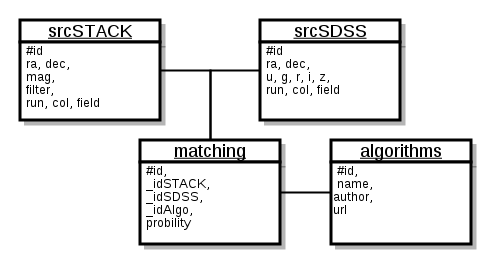
\includegraphics[width=0.9\textwidth]{img/bdd_star.png}
		\caption[Modèle relationnel en étoile]{Modèle relationnel en étoile pour stocker les sources identifiées par SDSS et le \stack{}, ainsi que les informations relatives aux algorithmes et l'association effectuée.}
		\label{fig:bdd_star}
	\end{figure}

Les deux tables contenant les sources ont une taille similaire $n$, par conséquent la table contenant les résultats de l'association contiendra $n$ données par nouvel algorithme si les algorithmes utilisés n'associent une source qu'à une seule source. Si un algorithme associe une source à plusieurs sources, ces données sont tout simplement stockées à l'aide de plusieurs identifiant unique dans notre base.


		\subsubsection{Modèle à colonnes variables}
% ^^^^^^^^^^^^^^^^^^^^^^^^^^^^^^^^^^^^^^^^^^^^^^^^^^^^^^^^^^^^^^^^^^^^^^
 
Il s'agit d'un modèle avec 3 tables. Comme précédement deux tables sont dédiées au stockage des sources, ainsi qu'une table pour les informations des algorithmes. Mais contrairement au modèle en étoile, on agit sur les deux tables contenant les sources en ajoutant une colonne par algorithme et en y stockant l'identifiant de la source associée. Ceci permet d'obtenir directement la liste des sources de l'autre base associées à une source.

Les informations sur ces tables est résumé dans la figure \ref{fig:bdd_colvar} sous la forme d'un diagramme.

	\begin{figure}[h]
		\centering
		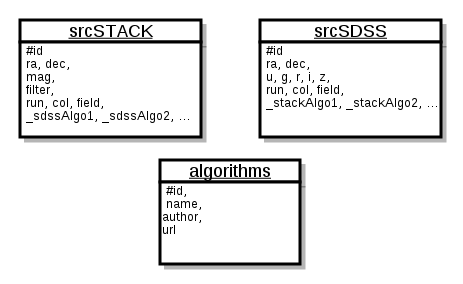
\includegraphics[width=0.9\textwidth]{img/bdd_colvar.png}
		\caption[Modèle relationnel à colonnes variables]{Modèle relationnel à nombre de colonnes variables pour stocker les sources identifiées par SDSS et le \stack{}, ainsi que les informations relatives aux algorithmes et l'association effectuée.}
		\label{fig:bdd_colvar}
	\end{figure}

Le problème est la modification du modèle relationnel qui peut entraîner une perte des données ou des lenteurs d'accès dû à l'ajout de données sur chaque ligne de la base.


% ======================================================================
\section{Jeu d'essai}
% ======================================================================

% ----------------------------------------------------------------------
	\subsection{Objectif}
% ----------------------------------------------------------------------

Il est courant d'effectuer des tests à partir de jeux d'essais, ceux-ci représente des cas standards d'utilisation ou permettent aussi de tester les limites d'un programme.

Dans notre cas le jeu d'essai est un ensemble de deux bases de données de sources. Une de ces bases est générée à partir de la première en ajoutant un bruit normal. Par conséquent chacune des sources à tester est généré à partir d'une de la base de référence, nos couples $(SDSS\,;\,Stack)$ sont prédéfinis. L'intérêt est donc de vérifier que nos algorithmes les associent correctement.

Après avoir fait tourner les programmes sur le jeu d'essai, nous meusurons trois quantités : les couples correctement formés, les couples erronés et les sources isolées. Il est important de maximiser la quantité des couples corrects. La quantité de minimiser en priorité est les couples erronés, il est préférable d'obtenir une absence d'information en obtenant une source seule plutôt qu'une mauvaise information.

\ 

À partir de ces résultats il est possible d'effectuer une ou plusieurs méthode d'optimisation en modifiant des paramètres d'entrée de nos algorithmes. La méthode la plus efficace est relativement simple à mettre en \oe{}uvre est la méthode du \emph{recuit-simulé}. L'absence de notion de voisinage dans le choix des paramètres complique l'utilisation d'une telle méthode car elle est conditionné par les tirages aléatoires des paramètres.

% ----------------------------------------------------------------------
	\subsection{Contrainte du jeu}
% ----------------------------------------------------------------------

Le jeu d'essai doit comporter certaines contraintes pour représenter au mieux la réalité. En effet il est possible qu'un programme associe plus facilement une source située en haut à gauche de la première, or si la génération aléatoire préconise ce placement, la détection d'un tel phénomène sera invisible. Il est donc important de posséder un bon générateur aléatoire.

En réalité en informatique il est très difficile d'avoir un générateur de nombres aléatoires (RNG pour \emph{random number generator}) puisque ces nombres sont issus d'un algorithme donc déterministes. On parle alors de générateurs de nombres pseudo-aléatoires (PRNG pour \emph{pseudo-random number generator}) car ces nombres sembles aléatoires. Une étude statistique permet de montrer que les générateurs de nombres pseudo-aléatoires possèdent une période et sont donc cycliques.

Le PRNG par défaut de \Cpp{} est considéré comme mauvais car ayant une courte période, sauf depuis \Cpp{}11 où un générateur plus performant a été implémenté. Ce nouveau générateur est l'algorithme de \emph{Mersenne Twister} découvert en 1997 et possédant une période de $2^{19937}-1$. Il est actuellement considéré comme un des meilleurs PRNG connu de par ses résultats au test de \emph{Diehard}, test des générateurs de nombres pseudo-aléatoires, et de par sa rapidité.

%% TODO: chercher une image montrant que certains PRNG sont mieux que d'autres

\ 

Il est aussi important de définir l'écart moyen et maximal prévu entre les données de SDSS et les résultats du \stack{} lors de la \DC{}. Le plus simple pour cela est d'utiliser les résultats déjà obtenu lors de mon précédent stage au LPC.

À partir de ces anciens résultats nous allons meusurer la largeur de la courbe en cloche obtenue, ainsi nous pouvons meusurer de façon empirique l'écart-type $\sigma$. Nous considèrerons que l'espérence est nulle. Ces deux informations permettent de définir une loi de probabilité normale $\mathcal{N}(\sigma,0)$. Cette loi de probabilité permet de créer un bruit gaussien sur les données de SDSS. Dans la pratique l'écart-type $\sigma$ est un vecteur de dimension 3, deux composantes pour l'ascension droite et la déclinaison, et une troisième pour la magnitude, obtenues à partir des mesures des écarts-types suivant ces trois paramètres.

	\begin{figure}[h]
		\centering
		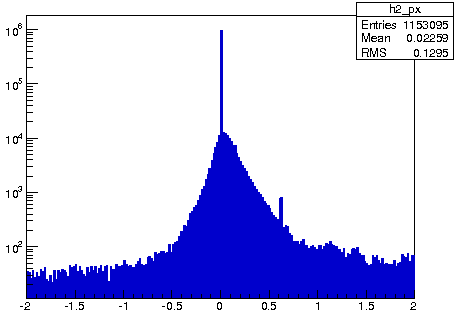
\includegraphics[width=0.9\textwidth]{img/mesuresigma.png}
		\caption[Mesure de l'écart-type à partir des anciens résultats]{Mesure de l'écart-type $\sigma$ à partir des résultats obtenus en août 2014.}
		\label{fig:mesuresigma}
	\end{figure}


% ======================================================================
\section{Recherche directe}
% ======================================================================

La première approche utilisée pour rechercher le plus proche voisin est une recherche dite diecte qui consiste à pour chaque point de la première base de données, on parcourt la seconde base, puis on compare le point de la première base et le point courant de la seconde.

	\begin{algorithm}
		\caption{Algorithme de recherche directe}
		\label{algo:direct-search}
		\begin{algorithmic}[1]
			\State $d_{min} \gets 100$; \Comment{Valeur arbitrairement grande de distance minimal d'initialisation}
			\For {$point_i$ dans la première base}
				\For {$point_j$ dans la deuxième base}
					\If {$d(point_i , point_j) < d_{min}$} \Comment{$d$ fonction de calcul de distance} \label{l:condi:algo:direct-search}
						\State $d_{min} \gets d(point_i , point_j)$;
					\EndIf
				\EndFor
			\EndFor
		\end{algorithmic}
	\end{algorithm}

Cet algoritme a une complexité en $\mathcal{O}(n^{2})$, il s'agit donc d'un algorithme relativement lent pour le problème à traiter, il n'est donc pas intéressant de l'utiliser sur un grand nombre de données. Malgré cela, cet algorithme est utilisé par sa modularité, en effet il est très simple de modifier la condition à la ligne \ref{l:condi:algo:direct-search} pour y prendre en compte la liste detous les paramètres que nous souhaitons prendre en compte.

\

L'optimisaton d'un tel algorithme peut se faire dans des cas particulier en effectuant un pré-traiement, d'une complexité parfois plus importante, permettant ensuite de réaliser un grand nombre de calcul rapidement. Il est donc nécessaire de trouver un juste milieu entre le temps d'éxécution du pré-traitement, et le gain obtenu par la suite au moment du traitement.

Il est aussi possible de lancer cette algorithme non pas sur toutes les données, mais sur un nombre restreint de données en découpant l'esapce en plusieurs morceaux. Cela équivaut à effectuer un partitionnement de l'espace.


% ======================================================================
\section[Arbres de partitionnement]{Structure d'arbres de partitionnement}
% ======================================================================

Certains algorithmes, ou approches algorithmiques, nécessite un partitionnement de l'espace des données pour diviser le travail et n'effectuer que des tâches élémentaires. Le pincipe de partition est proche d'une vision récursive, en effet on divise l'espace de travail tant que l'on ne se retrouve pas dans un cas simple que l'on sait traiter. Ceci permet de chercher le plus proche voisin mais aussi de créer des régions d'intéraction, cette dernière problématique ne nous intéressera pas ici. Le partitionnement est ensuite représenté par la structure d'un arbre comme une arborecense du partitionnement.

	\begin{figure}[h]
		\centering
		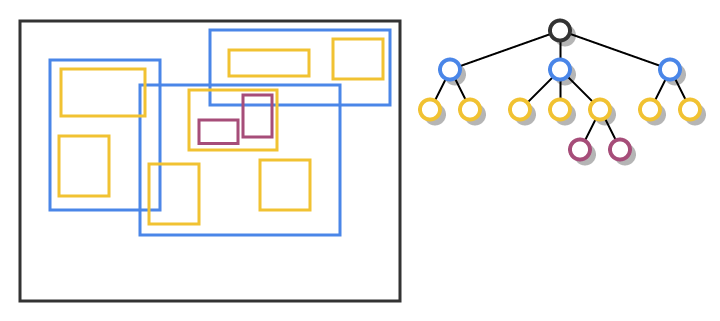
\includegraphics[width=0.9\textwidth]{img/rtree.png}
		\caption[Exemple de partitionnement et d'arbre associé]{Exemple d'arbre de partitionnement et de l'abre qui lui est assicié. Le principale intérêt est de travailler sur des ensembles de cardinal moins élevé, ou de mettre en valeur des espaces d'intéraction (\emph{R-tree} par exemple).}
	\end{figure}

Deux structures d'abre de partitionnement seront étudiées ici pour recherhcer le plus proche voisin, il s'agit du \emph{kd-tree} et du \emph{quad-tree}. Nous verrons les avantages et les inconvéniants des deux. Chaque n\oe{}ud de l'arbre représente une partition de l'espace, ses fils ses sous-partitions. Plusieurs partitionnements sont envisageables pour obtenir des divisons avec des propriétés plus ou moins intéressantes.


%-----------------------------------------------------------------------
	\subsection{Définition et propriété de l'espace de données}
%-----------------------------------------------------------------------

Avant de parler de l'algorithmie et des structures de données et il est important de parler des espaces dans lesquels nous allons travailler et de ce que nous voulons y faire. Les données que nous allons traiter sont des points dans un espace à 2 dimensions, et nous souhaitons rechercher le plus proche voisin. La définition du plus proche voisin n'est ici pas seulement d'ordre géométrique, en effet il est possible d'ajouter d'autres paramètres. La méthode choisi ici est dans un premier temps d'effectuer une discimination géométrique, puis le dernier choix selon d'autres critères.


Il est aussi possible de travailler en 3 dimensions, notre objectif est de travailler sur des sources lumineuses dans le ciel, par conséquent nous nous retrouvons avec deux dimensions d'espace (l'ascension droite et la déclinaison), mais il est aussi possible d'ajouter la magnitude (luminosité) comme dimension. Ainsi nous travaillerions dans un espace à 3 dimensions, dont 2 dimensions d'espace. Cette technique ne sera pas exploité ici car cela donne autant d'importance aux paramètres astrophysiques (ascension droite et déclinaison) qu'à un paramètre photométrique (magnitude) qui est fortement soumis aux erreurs de calibration et des conditions de mesure. Mathématiquement l'ajout de dimensions non spatiales (le temps ou un paramètre) n'est pas dérangeant et n'influe en rien la théorie. Ainsi il n'est pas rare de travailler en $n$ dimensions en fixant $n$ selon le besoin.

	\begin{figure}[h]
		\centering
			\subfloat[Espace à 2 dimensions.]{\label{fig:space2D}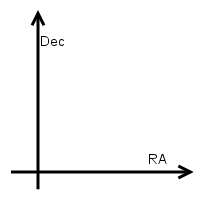
\includegraphics[height=4cm]{img/space2D.png}}
		\hspace{5pt}
			\subfloat[Espace à 3 dimensions.]{\label{fig:space3D}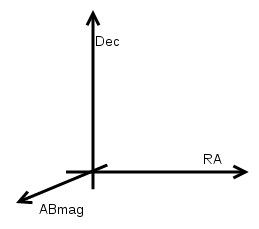
\includegraphics[height=4cm]{img/space3D.png}}
		\caption[Espace de travail à 2 ou 3 dimensions]{L'espace de travail peut être aussi bien à 2 qu'à 3 dimensions. L'exemple \ref{fig:space2D} montre un espace à 2 dimensions d'espaces ; l'exemple \ref{fig:space3D} montre un exemple d'espace à 2 dimensions d'espace et une de paramètres.}
		\label{fig:algoparsec}
	\end{figure}

\

La généralisation à $k$ dimensions est possible mais elle ne nous intéressera pas mais les différences des structures seront évoquées pour éveiller la curiosité du lecteur.

%-----------------------------------------------------------------------
	\subsection{Algorithme de construction}
%-----------------------------------------------------------------------

L'algorithme de construction de la structure du \emph{kd-tree} et du \emph{quad-tree} sont similaires, seule l'étape de division différe et est propre à chacune des structures. Le choix de la division implique des propriétés différentes sur les arbres générés. Cette étape sera détaillée en même temps que les différences des deux structures.

\

L'algorithme de construction est, sous sa forme la plus simple, récursif. Celui-ci est décrit dans l'algoritme \ref{algo:build-tree}.

	\begin{algorithm}
		\caption{Algorithme récursif de construction d'un arbre de partitionnement}
		\label{algo:build-tree}
		\begin{algorithmic}[1]
			\Function{Construire\_Arbre}{$espace$}
				\If{ nombre de points de l'espace = 0}
					\Comment{L'espace ne contient pas de source, impossible de diviser}
					\State \Return $espace$;
				\ElsIf{ nombre de point dans l'espace = 1}
					\Comment{L'espace ne contient plus qu'un point, il n'est plus nécessaire de diviser}
					\State \Return $espace$;
				\Else
					\Comment{Il faut diviser l'espace, et construire les sous espaces}
					\State \Return \Call{Construire\_Arbre}{ \textsc{Diviser\_Espace}($espace$) };
				\EndIf
			\EndFunction
		\end{algorithmic}
	\end{algorithm}

Le principe est simple, tant que l'espace contient plus d'une source on construit l'arbre sur les sub-divisions de l'espace. Quand il n'y a plus qu'une ou zéro source, on stope la division.


%-----------------------------------------------------------------------
	\subsection{Choix de la division}
%-----------------------------------------------------------------------

La différence entre la structure du \emph{quad-tree} et du \emph{kd-tree} est la méthode de divison de l'espace. Le partitionnement choisi possède des propriétés dépendante de cette méthode.

		\subsubsection{\emph{quad-tree}}
% ^^^^^^^^^^^^^^^^^^^^^^^^^^^^^^^^^^^^^^^^^^^^^^^^^^^^^^^^^^^^^^^^^^^^^^

La division du \emph{quad-tree} consiste à sub-diviser l'espace en quatre parties en prennant le milieu de chaque côté. Ceci permet de construire un arbre dont chaque n\oe{}ud possède 0 ou 4 fils.

La construction de cette arbre présente l'avantage d'être purement géométrique, ainsi il est possible d'effectuer un premier partitionnement pour utiliser un algorithme plus coûteux en complexité mais pouvant prendre en compte des paramètres plus fins d'association. En effet le plus proche voisin que nous cherchons n'est pas forcément le plus proche voisin géométrique mais le plus proche voisin en terme de ressemblance.

	\begin{figure}[h]
		\centering
		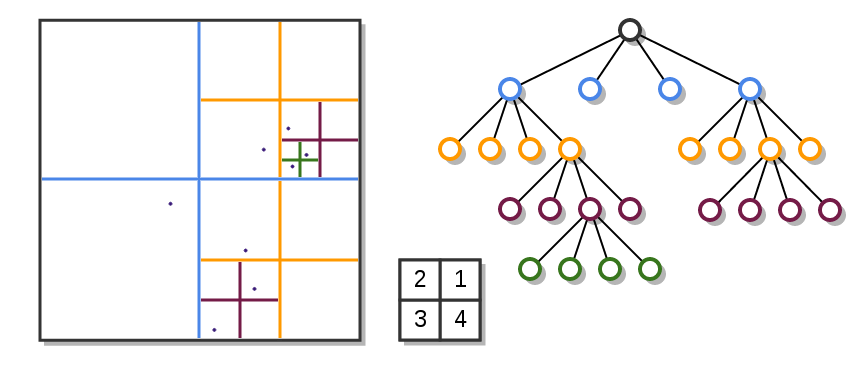
\includegraphics[width=0.9\textwidth]{img/quadtree.png}
		\caption[Relation entre la géométrie de l'ensemble et le \emph{quadtree} généré]{Relation entre la géométrie de l'ensemble (le placement des points dans l'espace), et la structure de données générée, le \emph{quadtree}. Chaque découpage est effectué avec une couleur différente pour voir son association avec l'arbre. La convention d'ordre des fils est celle des quadrants d'un repère orthonormé. On observe le découpage des sous-espaces tant qu'il n'y a pas zéro ou un élément.}
		\label{fig:quadtree}
	\end{figure}


Cette structure est généralisable facilement en 3 dimensions et portent le nom d'\emph{oct-tree}, chaque n\oe{}ud ne possède plus 4 mais 8 fils. Il est possible de passer en dimensions $k$ en divisant en 2 chaque axe, et ainsi obtenir $2^{k}$ sous-espace, donc $2^{k}$ fils à chaque n\oe{}ud.


Le problème de cette généralisation est la largeur et la profondeur de l'arbre obtenu, en effet si deux sources sont proches, il est parfois nécessaire d'effectuer un nombre important de divisions avant de réussir à séparer deux sources. C'est pour cette raison que cette algorithme ne sera utilisé que pour effectuer un premier partitionnement pour utiliser un algorithme plus lent sur des plus petites portions.


		\subsubsection{\emph{kd-tree}}
% ^^^^^^^^^^^^^^^^^^^^^^^^^^^^^^^^^^^^^^^^^^^^^^^^^^^^^^^^^^^^^^^^^^^^^^

La division du \emph{kd-tree} consiste à sub-diviser l'espace en tenant compte du nombre de points. En effet on remarque que le \emph{quad-tree} est très rarement équilibré, de nombreux n\oe{}uds ne servent pas, etc. Ces problèmes ont une cause commune qui est la division selon des critères géométriques sans tenir compte des données que l'espace contient. Ainsi la division du \emph{kd-tree} s'effectue suivant la médiane. Cette séparation permet d'obtenir deux sous-espaces contenant le même nombre de points plus ou moins 1 --- si l'espace contient un nombre impair de points.

Le problème de la médiane est que cette séparation s'effectue dans une liste, donc un espace à 1 dimension. La solution consiste à choisir à chaque itération une dimension selon laquelle nous effecturons la division. Ce choix s'effectue selon la parité de l'itération, si l'itération est pair nous effectuerons la division selon l'axe des $x$ (ascension droite dans notre cas), si l'itération est impair selon l'axe des $y$ (déclinaison).

	\begin{figure}[h]
		\centering
		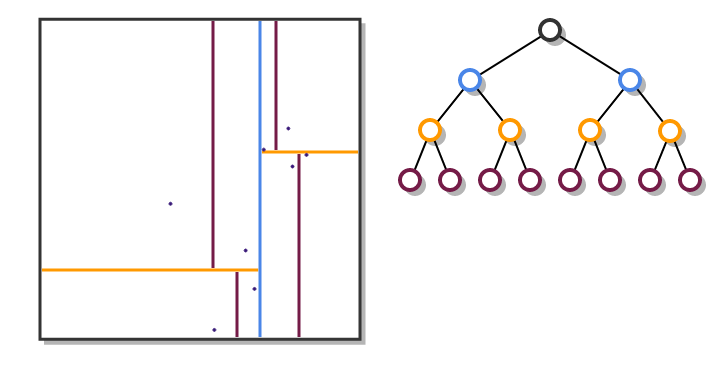
\includegraphics[width=0.9\textwidth]{img/kdtree.png}
		\caption[Relation entre la géométrie de l'ensemble et le \emph{kd-tree} généré]{Relation entre la géométrie de l'ensemble (le placement des points dans l'espace), et la structure de données générée, le \emph{kd-tree}. Chaque séparation divise l'espace en deux sous-espaces contenant un nombre égal de points. On remarque très facilement que l'arbre binaire est toujours équilibré grâce au découpage suivant la médiane.}
		\label{fig:kdtree}
	\end{figure}

Pour le cas de $k$ dimensions, le choix de la dimension s'effectue selon la congruence de l'itération modulo $k$, cela permet d'avoir une division régulière sur toutes les dimensions. La structure du \emph{kd-tree} évolue très bien au passage des dimensions supérieures puisqu'il s'agit toujours d'un arbre binaire dont la profondeur n'est que fonction du nombre de données. Quelque soit le nombre de dimensions la profondeur reste égale à $\log_{2}(n)$ où $n$ représente le nombre de points.



% ======================================================================
\section{Dérécursification}
% ======================================================================

L'algorithme \ref{algo:build-tree} est un algorithme dit récursif, cela signifie qu'il fait appelle à lui-même dans sa résolution. C'est le cas par exemple de la définition de la fonction factorielle.
	\begin{displaymath}
		\left\{\begin{tabular}{l}
			$n\,! = n \times (n-1)\,!$ \\
			$0\,!= 1$ \\
		\end{tabular}\right.
	\end{displaymath}
Lors de l'implémentation d'une telle fonction, celle-ci se rappelle elle-même jusqu'à un cas que l'on sait traiter c'est à dire factorielle de zéro. D'un point de vu informatique cela indique que nous ajoutons un appel de fonction dans la pile d'exécution. L'ajout d'information dans la pile d'exécution nuit à la performance mais aussi à la modularité du programme. Pour ces raisons il peut être intéressant de récursifier un algorithme. Cette technique revient à gérer soit même la pile d'exécution en ne sauvant pas tout l'appelle à la fonction mais seulement son résultat intermédiaire. Le résultat final est obtenu en dépilant les informations préalablement stockée dans la pile.


%-----------------------------------------------------------------------
	\subsection{Objectif}
%-----------------------------------------------------------------------

Notre algorithme est plus simple a comprendre sous sa forme récursive, et les seuls modifications que nous voulons apporter sont des limitations quant au nombre d'itérations. Ainsi l'aspect modulaire de la dérécursification ne nous intéresse pas, seul l'aspect performance nous intéresse.


